\documentclass[acmtocl,acmnow]{acmtrans2m}
\usepackage{amssymb}
\usepackage{amsmath}
\usepackage{url}
\usepackage{wrapfig}
\usepackage[usenames]{color}
\usepackage[dvips]{epsfig,psfrag}

%graphics
\newcommand{\ellipse}[1]{{\raisebox{-1ex}{\protect\psfrag{a}[][]{\small$#1$}%
\protect\includegraphics[width=10mm,height=5mm,clip]{vertex.eps}}}}
\newcommand{\Sourcevertex}{{\raisebox{-.2ex}{\includegraphics[width=3.5mm,clip]{sourcevertex.eps}}}}
\newcommand{\Sinkvertex}{{\raisebox{-.2ex}{\includegraphics[width=3.5mm,clip]{sinkvertex.eps}}}}
\newcommand{\sourcevertex}{{\raisebox{-.2ex}{\includegraphics[width=2.5mm,clip]{sourcevertex.eps}}}}
\newcommand{\sinkvertex}{{\raisebox{-.2ex}{\includegraphics[width=2.5mm,clip]{sinkvertex.eps}}}}

%names and CS terms
\newcommand{\entry}{entry}
\newcommand{\exit}{exit}
\newcommand{\Loop}{loop}
\newcommand{\EndLoop}{endloop}
\newcommand{\branch}{branch}
\newcommand{\EndBranch}{endbranch}
\newcommand{\basicblock}{basicblock}
\newcommand{\mfefninety}{mfef90}
\newcommand{\OpenAD}{OpenAD}
\newcommand{\OpenADFortTk}{OpenADFortTk}
\newcommand{\OpenAnalysis}{OpenAnalysis}
\newcommand{\OpenSixtyFour}{Open64}
\newcommand{\xaif}{XAIF}
\newcommand{\xaifBooster}{xaifBooster}
\newcommand{\whirl}{whirl}
\newcommand{\whirlToxaif}{whirl2xaif}
\newcommand{\whirlTof}{whirl2f}
\newcommand{\xaifTowhirl}{xaif2whirl}

%math
\newcommand{\R}{I\!\!R}
\newcommand{\bmC}{\mbox{\bf\em C}}
\newcommand{\bmf}{\mbox{\bf\em f}}
\newcommand{\bmg}{\mbox{\bf\em g}}
\newcommand{\bmI}{\mbox{\bf\em I}}
\newcommand{\bmJ}{\mbox{\bf\em J}}
\newcommand{\bmu}{\mbox{\bf\em u}}
\newcommand{\bmv}{\mbox{\bf\em v}}
\newcommand{\bmw}{\mbox{\bf\em w}}
\newcommand{\bmx}{\mbox{\bf\em x}}
\newcommand{\bmy}{\mbox{\bf\em y}}

%environments
\newcommand{\code}[1]{{\small\tt{#1}}}
\newcommand{\reffig}[1]{Figure~\ref{#1}}
\newcommand{\reffigs}[2]{Figures~\ref{#1}, \ref{#2}}
\newcommand{\refsec}[1]{Section~\ref{#1}}
\newcommand{\refeqn}[1]{(\ref{#1})}
\newcommand{\refcan}[1]{(C\ref{#1})}
\newtheorem{Can}{Canonicalization}

\markboth{Lots Of Authors et al.}{\OpenAD}

\title{\OpenAD: A tool for automatic differentiation 
of Fortran90 codes}

\author{PATRICK HEIMBACH, CHRIS HILL, DERYA OZYURT, CARL WUNSCH\\Massachusetts Institute of Technology\\
MIKE FAGAN, NATHAN TALLENT \\Rice University\\
MICHELLE STROUT, JEAN UTKE \\Argonne National Laboratory 
\and
UWE NAUMANN\\Rheinisch Westf\"alische Techinische Hochschule Aachen\\
{\color{Red}[ fix the ordering ]}
}

\begin{abstract}
The \OpenAD\ tool allows the evaluation of first and second order 
derivatives of functions defined by a program written in Fortran90/77. 
The derivative evaluation is performed by Fortran 90 code resulting from the 
analyses and transformation of the original program that defines the function of interest.
The code transformation follows the basic principles of automatic differentiation. 
In difference to most other automatic differentiation tools \OpenAD\ is 
built from components that permit an easy extension of the code transformations 
in a language indepdendent fashion. It uses code analysis results implemented 
in the \OpenAnalysis\ component. 
The interface to the language independent transformation 
engine is an xml abstract interface format, called \xaif\ that is  specified through an xml schema. 
The implemented transformation algorithms allow efficient derivative computations utilizing 
locally optimized cross country  sequences of vertex, edge and face elimination steps. 
Specifically for the generation of adjoint codes \OpenAD\ supports various code reversal 
schemes with hierachical checkpointing at the subroutine level. 
The Fortran specifive front and back end to this transformation engine is the \OpenSixtyFour\ based
\OpenAD\ Fortran tool kit, \OpenADFortTk.
\end{abstract}


\category{G.1.4}{Quadrature and Numerical Differentiation}{Automatic differentiation}
\category{D.3.4}{Processors}{Code generation, Compilers}
\category{F.3.2}{Semantics of Programming Languages}{Program analysis}
\category{G.1.6}{Optimization}{Gradient methods}

\terms{Algorithms, Performance}

\keywords{Automatic differentiation,  source transformation, adjoint compiler}

\begin{document}


\begin{bottomstuff} 
P.~Heimbach, C.~Hill, D.~Ozyurt, and C.~Wunsch, Massachusetts Institute of Technology, 
Boston, MA 02139;\newline
M.~Fagan, N.~Tallent, Rice University, 
Houston, TX 77251;\newline
M.~Strout, J.~Utke, Argonne National Laboratory, 
Argonne, IL 60439;\newline
U.~Naumann, Rheinisch Westf\"alische Techinische Hochschule Aachen, 
D-52056 Aachen, Germany;\newline
Funding for the ACTS project is provided by NSF under ITR contract OCE-0205590
for a three year period that started in September 2002.
\end{bottomstuff}
\maketitle

%#########################################################################################
\section{Introduction} \label{sec:Introduction}

The basic principles of automatic differentiation (AD), see also \refsec{ssec:ADIntro}, 
have been known for several decades \cite{wengert}
but only during the last 15 years the tools implementing AD have found a noticable use in 
optimization, data assimilation, and other applications in need of efficient and accurate 
derivative information. 
As a consequence of the wider use of AD 
a variety of tools have been developed that address specific 
application requirements or programming languages. 
The website {\tt www.autodiff.org} provides a good overview of the tools that 
are currently available. 
One may characterize two user groups of AD tools. On one side are the casual users 
with small scale problems applying AD mostly in a black box fashion and demanding 
minimal user intervention. 
On the other side are experienced AD users aiming for highly efficient 
derivative computations. Their need for efficiency is dictated by the 
computational complexity of models that easily reaches the limits of  current 
supercomputers. With the emphasis on efficiency some sacrifices on the support of 
language features are acceptable for this user group. 

One of the most demanding applications of AD is the computation of gradients for 
data assimilation on large scale models used in oceanography and climate research. 
An evaluation of the available tools revealed some shortcomings from the perspectives 
of the tool users as well as the tool developers. 

From  the AD tool  users point of view ... 
{\color{Red} [ FILL IN ] } 

From the AD tool developers point of view ...
{\color{Red} [ FILL IN ] } 

These issues became the motivation for the 
Adjoint Compiler Technology \& Standards (ACTS) project\footnote{ 
see {\tt www.stce.rwth-aachen.de/ACTS}
}. 
This project is a collaborative
research and development effort between MIT, Argonne National Laboratory, 
Univeristy of Chicago, and Rice University. 
It focusses on  next-generation tool development and 
application of AD to problems in oceanography and chemical engineering.
The main result of this effort is an infrastructure for the language independent 
development and use of AD algorithms. 
\OpenAD\ is the Fotran90 incarnation of the infrastructure.\footnote{
The C/C++ oriented ADIC version 2.0 is based on the same infrastructure and can be found
at {\tt www.mcs.anl.gov/adicserver}.
}
\begin{wrapfigure}{r}{6cm}
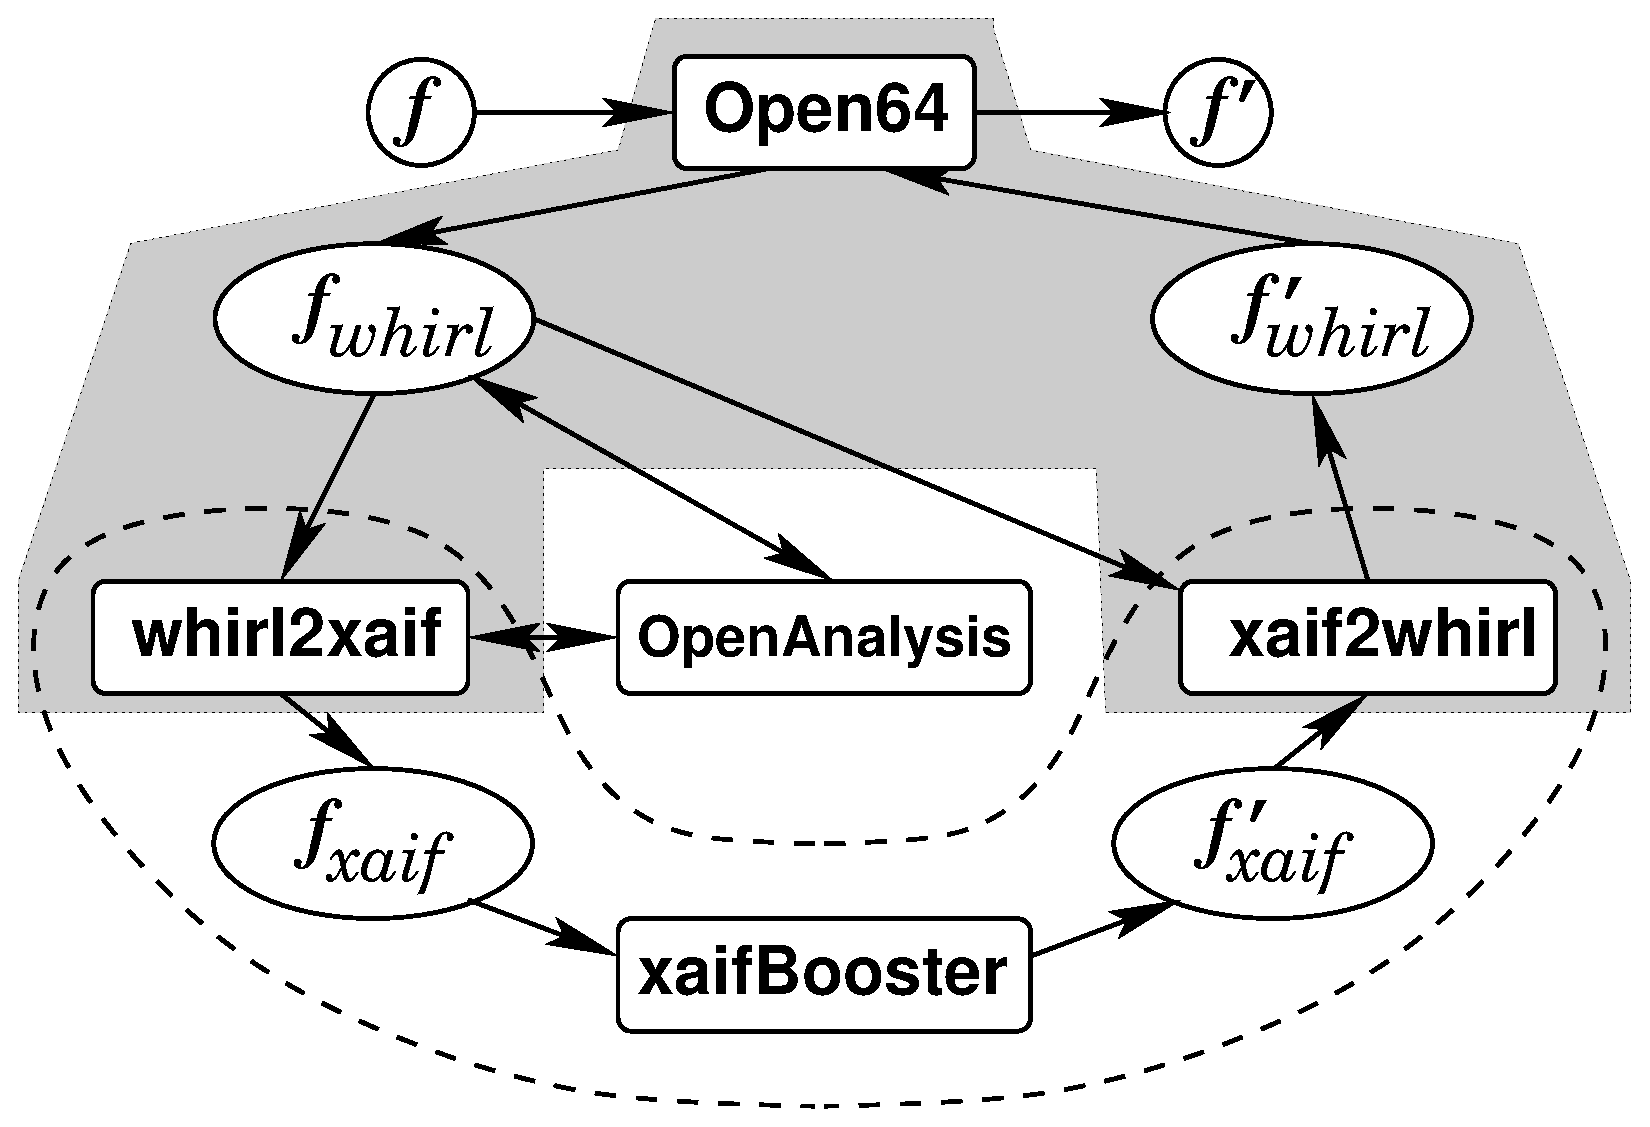
\epsfig{file=overview.eps,width=6cm}
\caption{\OpenAD\ components and pipeline} \label{fig:overview}
\end{wrapfigure}
The collaboration  of the \OpenAD\  components is illustrated in 
\reffig{fig:overview}
The \OpenSixtyFour\ front-end performs a lexical, 
syntactic, and semantic analysis and produces an 
intermediate representation of $F$ in the so-called \whirl\ format.
\OpenAnalysis\ is used to build call and control flow graphs and  perform 
code analyses such as alias, activity, side-effect analysis.
This information is used by 
\whirlToxaif\ to construct a representation of the numerical core of $F$ in
\xaif\ format shown as $F_{xaif}$.  
A differentiated version of $F_{xaif}$ is derived by an 
algorithm that is implented in \xaifBooster\ and is again respresented 
\xaif\ as $F'_{xaif}$.
The information in $F'_{xaif}$ and the original $F_{\whirl}$ are used by 
\xaifTowhirl\ to construct a 
\whirl\ representation $F'_{\whirl}$ of the differentiated code. 
The unparser of 
\OpenSixtyFour\ transforms $F'_{\whirl}$ into Fortran90, thus completing
the semantic transformation of a program $F$ into
a differentiated program $F'$.
The dotted line encloses the language specific front-end that can potentially
be replaced by front-ends for languages other than Fortran. 
For example, an 
effort running parallel to the ACTS project at Argonne National Laboratory is 
developing a new version of ADIC \cite{HoNo01} by coupling a C/C++ 
front-end 
based on an EDG parser ({\tt www.edg.com}) and uses ROSE in combination with SAGE~3 ({\tt www.llnl.gov/CASC}) as internal representation
with \OpenAD.

This paper discusses the components of \OpenAD,
including the underlying design decisions, algorithmic aspects, and
numerical results.
 
%#########################################################################################
\section{AD Concepts}\label{sec:ADIntro}

In this section we introduce the terminology we will refer to throughout 
this paper. We will also introduce a number of canonicalizations 
that are required to simplify the theoretical and practical 
aspects of the code transformation in \OpenAD.

A detailled introduction to AD can be found in \cite{Gri00}. 
We would also like to refer the reader to the proceedings of four conferences 
on AD \cite{CG91,BBCG96,CFG+01,BCH+05}.

We assume a vector valued function $\bmy=\bmf(\bmx): \R^n\mapsto \R^m$ that is implemented 
as a computer program in a language such as Fortran, C, or C++. 
The computer program 
induces a {\em call graph} (CG) \cite{Aho}
whose vertices are subroutines and whose edges 
represent calls potentially made during the computation of $\bmy$ for particular 
values of $\bmx$. 
Every subroutine consists of a {\em control flow graph} (CFG) that 
represents the typical control flow constructs such as \entry, \exit, \Loop, \branch, 
and \basicblock. 
A \basicblock\ consists of a sequence of assignments and subroutine calls. 
In the following we assume some canonicalizations are performed. 
These canonicalizations are implemented in the front end discussed in 
\refsec{sssec:Canonicalization}.
\begin{Can} \label{can:funcToSub}
All constructs occuring in \basicblock\ that are neither assignments nor subroutine calls (such as function calls, built-in I/O statements) 
are canonicalized into subroutine calls.
\end{Can}
\begin{Can} \label{can:assignSideEffectFree}
An assignment effects a single variable on the left-hand side and 
the right-hand-side expression is side-effect free.
\end{Can}
\begin{Can} \label{can:assignElemental}
The right-hand-side expression consists only of elemental operations $\phi$ typically 
defined in a programming language as built-in operators and intrinsics.
\end{Can}
\begin{Can} \label{can:assignFunction}
User defined functions and calls to these functions in right-hand-side expressions 
are canonicalized to subroutined calls.
\end{Can}
Without loss of generality we can assume that an evaluation of $\bmf(\bmx)$ for  
a particular value of $\bmx$ can be represented by a sequence of 
elemental operations $v_j=\phi_j(\ldots,v_i,\ldots)$. 
The $v_i$ represent the vertices $\in V$ in the correspong corresponding computational 
graph $G=(V,E)$. The edges $(i,j)\in E$ in this graph are the direct dependencies 
$v_i\prec v_j$ implied by the elemental $v_j=\phi_j(\ldots,v_i,\ldots)$.

The elemental operations $\phi$ are differentiable on open subdomains. 
Each edge $(i,j)\in E$ has an attached local partial derivative 
$c_{ji}=\frac{\partial v_j}{\partial v_i}$. 
The central principle of AD is 
the application of the chain rule to the elemental $\phi$, that is 
multiplications and additions of the  $c_{ji}$.  

Because the code for a $\bmf$ generally contains control flow constructs there is no 
single $G$ that represents the computation of $\bmf$ for all possible values of $\bmx$.
In practice, \OpenAD\ considers subgraphs constructed 
from the contents of a \basicblock.
In the following we illustrate the prinicpal approach with the use 
of a toy example.  
Line numbers have been added for simpler referencing within the text.
\begin{wrapfigure}{l}{.5\linewidth}
\begin{tabbing}
\hspace{.6cm}{\footnotesize \bf 01}\hspace{.5cm} {\tt y(k)=sin(x(1)*x(2)); k=k+1} \\
\hspace{.6cm}{\footnotesize \bf 02}\hspace{.5cm} {\tt if} \={\tt (mod(k,2) .eq. 1) then } \\
\hspace{.6cm}{\footnotesize \bf 03}\hspace{.5cm} \>{\tt y(k)=2*y(k-1)}  \\
\hspace{.6cm}{\footnotesize \bf 04}\hspace{.5cm} {\tt else } \\
\hspace{.6cm}{\footnotesize \bf 05}\hspace{.5cm} \>{\tt do} \={\tt i=1,k } \\
\hspace{.6cm}{\footnotesize \bf 06}\hspace{.5cm} \>\>{\tt t1=x(1)+x(2) } \\
\hspace{.6cm}{\footnotesize \bf 07}\hspace{.5cm} \>\>{\tt t2=t1*sin(x(1)) } \\
\hspace{.6cm}{\footnotesize \bf 08}\hspace{.5cm} \>\>{\tt x(1)=cos(t1*t2) } \\
\hspace{.6cm}{\footnotesize \bf 09}\hspace{.5cm} \>\>{\tt x(2)=-sqrt(t2) } \\
\hspace{.6cm}{\footnotesize \bf 10}\hspace{.5cm} \>{\tt end do } \\
\hspace{.6cm}{\footnotesize \bf 11}\hspace{.5cm} {\tt end if } \\
\hspace{.6cm}{\footnotesize \bf 12}\hspace{.5cm} {\tt y(k)=y(k)+x(1)*x(2) } 
\end{tabbing}
\caption{Toy example code}\label{fig:toy}
\end{wrapfigure}
The CFG resulting from the above code is depicted in 
\reffig{fig:cfg}(a).
The assignment statements are contained in the {\basicblock}s B(2,3,4,6,12).
For instance, 
the statements  in the lines 06--09 form the loop body, \basicblock\ B(6).
As B(6) is executed
{\tt k} times it may be worth putting
additional effort into the optimization of the derivative code 
generated for B(6).
\begin{figure}[ht]
\centering
\begin{tabular}{ccc}
\epsfig{file=cfg_ts.ps,width=.303\textwidth} &
\epsfig{file=cfg_tape.ps,width=.303\textwidth} &
\epsfig{file=cfg_adj.ps,width=.31\textwidth} \\
\em (a) & \em (b) & \em (c)
\end{tabular}
\caption{CFG of \reffig{fig:toy} (a) original code, (b) tangent linear model, (c) adjoint model}\label{fig:cfg}
\end{figure}
For B(6) the corresponding computational graph $G$  is depicted in
\reffig{fig:elims}(a).  

Like most of the AD literature we follow a specific numbering scheme for the vertices $v_i$.
heWe presume $q$ intermediate values
$v_j = \phi_j(\ldots,v_i,\ldots), v_j\in Z$
for $j=1,\ldots,q+m$ and $h,i=1-n,\ldots,q,$ $j>h,i$. 
The $n$ {\em independent}
variables $x_1,\ldots,x_n$ correspond to 
$v_{1-n},\ldots,v_0, v_i\in X$. 
We consider the 
computation of derivatives of the {\em dependent} variables 
$y_1,\ldots,y_m$ represented by $m$ variables $v_{q+1},\ldots,v_{q+m}, v_j\in Y$
with respect to the independents. The depdendencies $v_i<v_j$ implies $i<j$. 
The {\em forward mode} of AD propagates directional derivatives
as 
\begin{equation} \label{eqn:fm}
\dot{v}_j= \sum\limits_i\frac{\partial \phi_j}{\partial v_i}\dot{v}_i 
\quad \text{for}~~j=1,\ldots,q+m.
\end{equation} 
In {\em reverse mode} we compute adjoints of the arguments of the $\phi_j$
as a function of local partial derivatives and the 
adjoint of the variable on the left-hand side
\begin{equation} \label{eqn:rm}
\overline{v}_i= \sum\limits_j\frac{\partial \phi_j}{\partial v_i}\dot{v}_i 
\quad \text{for}~~j=1,\ldots,q+m.
\end{equation} 
In practice the sum in \refeqn{eqn:rm} is split into individual increments 
associated with each statement in which $v_i$ occurs as an argument 
$\overline{v}_i=\overline{v}_i+\overline{v}_j * \frac{\partial \phi_j}{\partial v_i}$.

Equations \refeqn{eqn:fm} and \refeqn{eqn:rm} can be used to accumulate 
the (local) Jacobian $\bmJ_{B(6)}$
of B(6), see also \refsec{ssec:elimMeth}. 
For a sequence of $l$ {\basicblock}s that are part of 
a path through the CFG for a particular value of $\bmx$ the 
equations~(\ref{eqn:fm}) and (\ref{eqn:rm}) can be generalized as follows:
\begin{equation} \label{eqn:bbfm}
\dot{\bmy}_j=\bmJ_j \dot{\bmx}_j \quad \text{for}~~j=1,\ldots,l
\end{equation} 
and 
\begin{equation} \label{eqn:bbrm}
\bar{\bmx}_j=\bmJ^T_j \bar{\bmy}_j \quad \text{for}~~j=l,\ldots,1\quad ,
\end{equation} 
where $\bmx_j = (x^j_i \in V :  i=1,\ldots,n_j)$ and
$\bmy_j = (y^j_i \in V : i=1,\ldots,m_j)$ are the inputs and outputs of the 
{\basicblock}s
respectively. 
In forward mode a sequence of 
products of the local Jacobians $\bmJ_j$ 
with the directions $\dot{x}_j$ 
are propagated forward in the direction of the flow of control, for 
instance simultaneouly to the computation of $\bmf$.
 
In reverse mode products of the transposed
Jacobians $\bmJ^T_j$ with adjoint vectors $\overline{\bmy}_j$
are propagated reverse to the direction of the flow of control. 
%%%%%%%%%%%%%%%%%%%%%%%%%%%%%%%%%%%%%%%%%%%%%%%%%%%%%%%%%%%%%%%%%%%%%%%%%%%%%%
\subsection{CFG Reversal} \label{ssec:cfgReversal}
In order to find the corresponding path to the reversed control flow graph 
we have to record certain essential information in an augmented CFG,
for our toy example see \reffig{fig:cfg}(b).
The augmented CFG  keeps track of which branch was taken and counts how often a loop was 
executed.  
This information is pushed on  a stack and popped from that stack during the 
reverse sweep.  
In the example in \reffig{fig:cfg}(b) the extra {\basicblock}s pBT and pBF push 
either a ``true'' or ``false'' value onto the stack depending on the branch. 
In iLc we initialize a loop counter, increment in +Lc, and push the final 
count in pLc. 

\reffig{fig:cfg}(c) shows the reversed CFG for our toy example. 
The parenthesized numbers in the node labels align the 
node transformation to \reffig{fig:cfg}(a). 
The \exit\ node becomes 
the \entry, \Loop\ becomes \EndLoop, \branch\ beomes \EndBranch, and vice versa. 
Each \basicblock\  B is replaced with its reversed version B'.  
Finally, to find the proper path through this reversed CFG we need to retrieve 
the information recorded in  \reffig{fig:cfg}(b). The extra nodes pB and pLc 
pop the branch information and the loop counter respectively.  
We enter the branch and execute the loop as indicated by the recorded information. 
The process of the control flow reversal is described in detail in 
\cite{NULF04CFR}. 
%%%%%%%%%%%%%%%%%%%%%%%%%%%%%%%%%%%%%%%%%%%%%%%%%%%%%%%%%%%%%%%%%%%%%%%%%%%%%%
\subsection{Elimination Methods} \label{ssec:elimMeth}
Let $\bmf$ represent a single \basicblock\ that is subject to preaccumulation
as outlined in the previous section.
For notational simplicity and without loss of generality we assume that the 
dependent variables are mutually independent. 
This situation can always be
reached by introducing auxiliary assignments.
\begin{figure}[ht]
\centering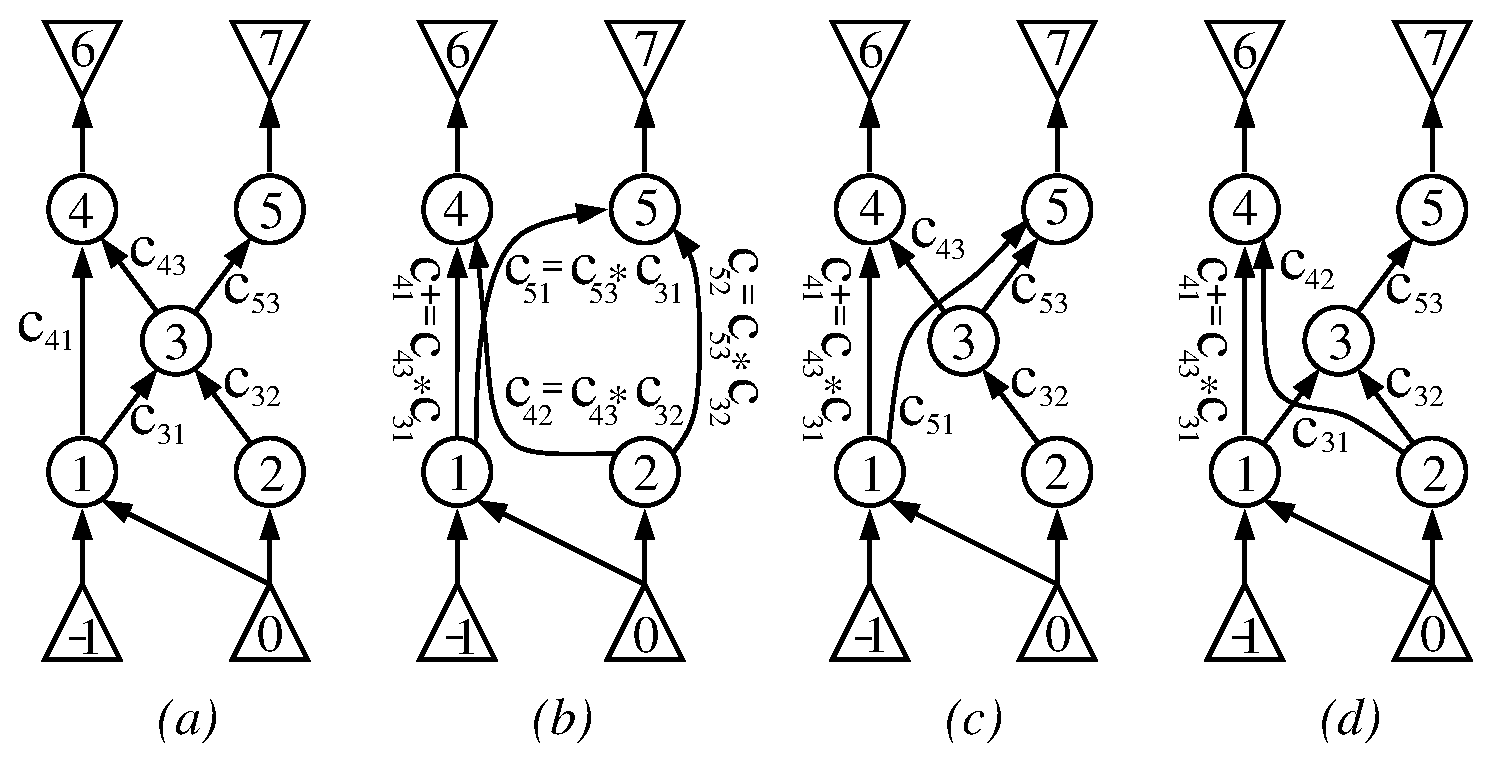
\epsfig{file=elims.eps,width=.7\linewidth}
\caption{
(a) Computational graph $G$ for \refeqn{eqn:sampleCode}, 
(b) eliminate vertex 3 from $G$, 
(c) front eliminate edge $(1,3)$ from $G$, 
(d) back eliminate edge $(3,4)$ from $G$} 
\label{fig:elims}
\end{figure}
In \reffig{fig:elims}~(a) we show the DAG for B(6) from \reffig{fig:toy}. 
It represents a decomposition of the code into a sequence assignments of
the results of the elemental operations $\phi$ to unique intermediate 
variables,
for example,
\begin{equation}\label{eqn:sampleCode}
\begin{split}
 v_1&=v_{-1}+v_0;~v_2=\sin(v_0);~v_3=v_1+v_2;~v_4=v_1*v_3; \\
v_5&=\sqrt{v_3};~v_6=\cos(v_4);~v_7=-v_5 \quad .\\
\end{split}
\end{equation}
The edges $(i,j)\in E$ are labeled with partial derivatives
$c_{ji}$, for instance, in the 
example we have $c_{64}=-\sin(v_4)$.
Jacobian preaccumulation can be interpreted as eliminations in $G$.
The graph-based elimination steps are categorized in vertex, edge, and face 
eliminations. 
In $G$ a vertex $j \in V$ is eliminated by connecting its predecessors with
its successors \cite{GrRe91}.
An edge $(i,k)$ with
$i \prec j$ and $j \prec k$ is labeled with
$c_{ki}+c_{kj} \cdot c_{ji}$ if it existed before the elimination of $j.$
We say that {\em absorption} takes place.
Otherwise, $(i,k)$ is generated as {\em fill-in} and labeled
with $c_{kj} \cdot c_{ji}$
The vertex $j$ is removed from
$G$ together with all incident edges. 
\reffig{fig:elims}~(b) shows the result of eliminating vertex $3$
from the graph in \reffig{fig:elims}~(a).

An edge $(i,j)$ is {\em front eliminated} by connecting $i$ with all successors
of $j$, followed by removing $(i,j)$ \cite{ElimTechAD2000}.
The corresponding structural modifications of the c-graph in
\reffig{fig:elims}~(a) are shown in
\reffig{fig:elims}~(c) for front elimination of $(1,3).$
The new edge labels are given as well.
Edge-front elimination eventually leads to intermediate vertices in $G$
becoming
{\em isolated}; that is, these vertices no longer have predecessors.
Isolated vertices are simply removed from $G$ together
with all incident edges.

Back elimination of an edge
$(i,j) \in E$ results in connecting all predecessors of $i$
with $j$ \cite{ElimTechAD2000}.
The edge $(i,j)$ itself is removed from $G.$
The back elimination of $(3,4)$ from the graph in \reffig{fig:elims}~(a) 
is illustrated in \reffig{fig:elims}~(d). 
Again, vertices can become isolated as a result of edge-back elimination
because they no longer have successors.
Such vertices are removed from $G.$

Numerically the elimination is the application of 
the chain rule, that is, a sequence of {\em fused-multiply-add} (fma) operations
\begin{equation}\label{eqn:fma}
c_{ki}=c_{ji}*c_{kj}\hspace*{1ex}(+c_{ki}) \hspace*{2ex}\gets \mbox{optional}
\end{equation}
where the additions take place in the case of absorption or fill-in is created 
as described above.

Aside from special cases a single vertex or edge elimination will result in more
than one fma. {\em Face elimination} was introduced 
as the elimination operation with the finest granularity of exactly 
one multiplication\footnote{Additions are not necessarily directly coupled.} 
per elimination step.

Vertex and edge elimination steps have an 
interpretation in terms of vertices and edges
of $G$, whereas face elimination is performed on 
the corresponding directed line graph $\cal G.$
Following \cite{ElimTechMP}, we define the directed line graph $\cal G=(V,E)$ 
corresponding to $G=(V,E)$ as follows:
$${\cal V}=
\{\ellipse{i,j} : (i,j)\in E\} \cup 
\{\ellipse{\sourcevertex,j}:v_j \in X\} \cup 
\{\ellipse{i,\sinkvertex}:v_i \in Y\}$$ and 
\begin{align*}
{\cal E}&=\{(\ellipse{i,j},\ellipse{j,k}): (i,j),(j,k) \in E\} \\
&\cup \{(\ellipse{\sourcevertex,j},\ellipse{j,k}): v_j\in X \land (j,k)\in E\} \\
&\cup \{(\ellipse{i,j},\ellipse{j,\sinkvertex}): v_j\in Y \land (i,j)\in E\} 
\quad . \\
\end{align*}
That is, 
we add a source vertex \Sourcevertex\ and a sink vertex 
\Sinkvertex\ to $G$ connecting all independents to \Sourcevertex\
and all dependents to \Sinkvertex. $\cal G$ has   
a vertex $ v \in \cal V$ for each edge in the extended $G$, 
and $\cal G$ has an edge $ e \in \cal E$ for each 
pair of adjacent edges in $G$. \reffig{fig:face_elims} gives an 
example of constructing the directed line graph in (b) from the graph in (a).   
All intermediate vertices $\ellipse{i,j} \in \cal V$ inherit the labels  
$c_{ji}$. In order to formalize face elimination, it is advantageous to move away
from the double-index notation and use one that is based on a topological
enumeration of the edges in $G.$ Hence, ${\cal G}=({\cal V}, {\cal E})$ 
becomes a DAG with ${\cal V} \subset I\!\!N$ and
${\cal E} \subset I\!\!N \times I\!\!N$ and
certain special properties.
The set of all predecessors of $j \in {\cal V}$ is denoted as $P_j.$ 
Similarly, $S_j$ denotes the set of its successors in $\cal G.$ 
A vertex 
$j \in \cal V$ is called {\em isolated} if either 
$P_j=\emptyset$ or
$S_j=\emptyset.$ 
Face elimination is defined in \cite{ElimTechMP}
between two incident intermediate vertices $i$ and $j$ in $\cal G$ as follows:
\begin{enumerate}
\item If there exists a vertex $k \in \cal V$ such that $P_k = P_i$ and
$S_k = S_j,$ then
set $c_k = c_k + c_j c_i$ {\em (absorption)};
else ${\cal V}={\cal V} \cup \{k'\}$ with a new vertex $k'$ such that
$P_{k'} = P_i$ and $S_{k'} = S_j$
{\em (fill-in)} and labeled with $c_{k'} = c_j c_i.$
\item Remove $(i,j)$ from $\cal E.$
\item Remove $i \in \cal V$ if it is isolated. Otherwise, if there exists a vertex $i' \in \cal V$ such that
$P_{i'} = P_i$ and $S_{i'} = S_i,$ then
\begin{itemize}
\item set $c_i=c_i + c_{i'}$ {\em (merge)};
\item remove $i'.$
\end{itemize}
\item Repeat Step 3 for $j \in \cal V.$
\end{enumerate}
In \reffig{fig:face_elims}~(c) we show the elimination of $(i,j) \in \cal E$,
where $i=\ellipse{1,3}$ and $j=\ellipse{3,4}$.

\begin{figure}
\centering
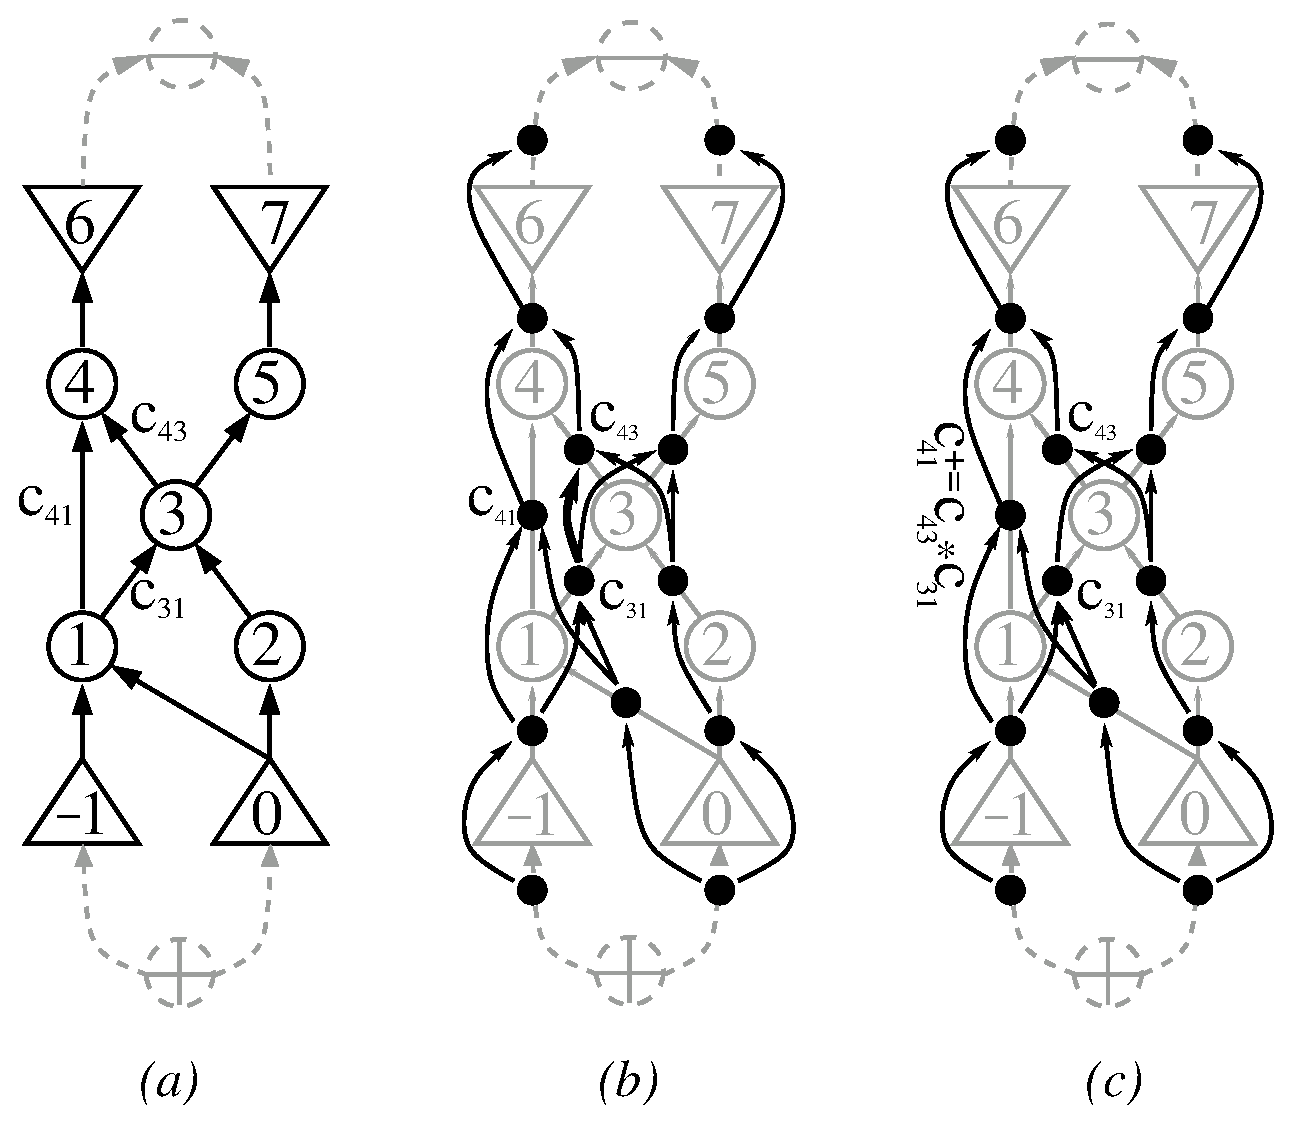
\epsfig{file=face_elims.eps,width=.65\linewidth}
\caption{
(a) $G$ extended, 
(b) $\cal G$ overlaid, 
(c) face elimination 
}
\label{fig:face_elims}
\end{figure}
A complete face elimination sequence $\sigma_f$ yields a tripartite 
directed line graph $\sigma_f({\cal G})$ that can be back transformed into 
the bipartite graph representing the Jacobian $\bmf'$.
We note that any $G$ can be transformed into the 
corresponding $\cal G$ but that a back transformation 
generally is not  possible once face elimination steps have been applied. 
Therefore, face eliminations cannot precede vertex and edge 
eliminations.

In a source transformation context of \OpenAD\ the operations \refeqn{eqn:fma} are 
expressed as actual code, the Jacobian accumulation code. For the 
B(6) from our toy example in \reffig{fig:toy} the code computing 
the local partials in conjunction with the function value, see \refeqn{eqn:sampleCode}, 
is shown in 
\reffig{fig:toyAndPartials}.
\footnote{
For better readability we write the indices of the $c_{ji}$ with commas.
} 
\begin{wrapfigure}{l}{.5\linewidth}
\begin{minipage}{\linewidth}
\begin{align*}
 v_1&=v_{-1}+v_0;~c_{1,-1}=1;~c_{1,0}=1; \\
 v_2&=\sin(v_0);~c_{2,0}=\cos(v_0); \\
 v_3&=v_1+v_2;~c_{3,1}=1;~c_{3,2}=1; \\
 v_4&=v_1*v_3;~c_{4,1}=v_3;~c_{4,3}=v_1; \\
 v_5&=\sqrt{v_3};~c_{5,3}=(2\sqrt{v_3})^{-1}; \\
 v_6&=\cos(v_4);~c_{6,4}=-\sin(v_4); \\
 v_7&=-v_5;~c_{7,5}=-1;
\end{align*}
\end{minipage}
\caption{Code for \refeqn{eqn:sampleCode} and the $c_{ji}$}\label{fig:toyAndPartials}
\end{wrapfigure}
Now the operations induced by the eliminations on the graph can 
be expressed in terms of the auxiliary variables $c_{ji}$.
For our example, a forward vertex elimination, that is, the elimination
sequence (1,2,3,4,5) in $G$ (\reffig{fig:elims}), leads to the
following Jacobian accumulation code.
{
%\small
\begin{align*}
1:\quad  &c_{3,-1}=c_{3,1} * c_{1,-1};~c_{3,0}=c_{3,1} * c_{1,0};~c_{4,-1}=c_{4,1} * c_{1,-1};~c_{4,0}=c_{4,1} * c_{1,0}; \\
2:\quad  &c_{3,0}=c_{3,2} * c_{2,0}+c_{3,0}; \\
3:\quad  &c_{4,-1}=c_{4,3} * c_{3,-1}+c_{4,-1};~c_{4,0}=c_{4,3} * c_{3,0}+c_{4,0};~c_{5,-1}=c_{5,3} * c_{3,-1}; \\
&c_{5,0}=c_{5,3} * c_{3,0}; \\
4:\quad  &c_{6,-1}=c_{6,4} * c_{4,-1};~c_{6,0}=c_{6,4} * c_{4,0}; \\
5:\quad  &c_{7,-1}=c_{7,5} * c_{5,-1};~c_{7,0}=c_{7,5} * c_{5,0} \quad .
\end{align*}
}


%#########################################################################################
\section{\OpenAD\ components}
\OpenAD\  is built on components that belong to a framework aimed at 
code transformation of numerical programs. 
The components are tied together either via programmatic interfaces or they 
communicate via the \xaif. The transformation of the source code follows the 
pipeline shown in \reffig{fig:overview}. 
The following sections explain the role and inner workings of the various 
components in greater detail. 

%-----------------------------------------------------------------------------------------
\subsection{\OpenADFortTk\ - the Fortran~90 Front-End}

The main target application of the ACTS project is the MIT general
circulation model (MITgcm) \cite{mars-eta:97b,mars-eta:97a}.
It is mostly implemented in Fortran~77 to permit maintenance of an
efficient and correct adjoint as the code evolves \cite{HHG02}. Future
development will increasingly add Fortran~90 features.  The
\OpenADFortTk\ (OpenAD Fortran Toolkit) 
component covers the
Fortran-specific features of the OpenAD system. Throughout this
paper, we use ``front-end'' as a synonym for \OpenADFortTk.

In spite of the appellation ``front end'', \OpenADFortTk\ subcomponents
operate at several stages of the pipeline in the following order.
	
   \begin{enumerate}	
     \item \mfefninety is a compiler front-end in the classical sense that parses
       Fortran and generates an intermediate representation (IR)
       in the \whirl\ language

     \item The {\em canonicalizer} converts  
        programming constructs into the canonical form required by 
	\refcan{can:funcToSub} - \refcan{can:assignFunction}. 
	This component modifies \whirl\ in core.

     \item \whirlToxaif\ is a bridge component that
        \begin{itemize}
           \item drives the various program analyses (see \refsec{ssec:openanalysis}),
        
           \item filters out program statements that are not in the
                 computational core of the language, and 

           \item converts the program analyses and core computational
                 statements from \whirl\ into \xaif.
        \end{itemize}

     \item \xaifTowhirl\ is bridge component that converts the 
        differentiated program represented in \xaif\ 
        to a \whirl\ representation.

     \item \whirlTof\ is the ``unparser'' that converts \whirl\ to
        Fortran.

     \item The {\em postprocessor} is the  final part of the transformation that
        performs template expansion as well as inlining substitutions.

   \end{enumerate}

Both \mfefninety\ and \whirlTof\ are part of the Open64 project.

In the following we will explain the 
subcomponents in more detail. 

%-----------------------------------------------------------------------------------------
\subsubsection{\OpenSixtyFour\ components} \label{sssec:mfef}
The \OpenSixtyFour\ project supplies 2 elements for the front end, 
\mfefninety and \whirlTof

To ensure robustness of the AD tool, we sought industrial strength
programming-language-dependent components.  We chose the Center for
High Performance Software Research's (Rice University) \OpenSixtyFour\
compiler \cite{open64Web}, 
a multi-platform version of the SGI Pro64/Open64 compiler
suite, originally based on SGI's commercial MIPSPro compiler.  
\OpenSixtyFour\'s Fortran
front end, \mfefninety, is a classical compiler parser that reads Fortran
source and converts it to an intermediate language called \whirl.  
A companion tool, \whirlTof, unparses \whirl\ back to Fortran source
code.  The \whirl\ representation, 
which resembles a typical abstract syntax tree, has been
designed to enable good optimization for high performance computing in
Fortran, C, and C++. See \cite{whirl-stuff} for more details about the
intermediate language. 
HiPerSoft's main contribution to the \OpenSixtyFour\ 
community has been extending the infrastructure to support
source-to-source transformations; thus, it has invested significant
effort in the \whirlTof\ unparser.

The \OpenAD\ project contributed some development of the pragma /
directive mechanism in the Open64 components.

{\color{Red} [ These pragmas are ...  They  are used ....

note: we will refer to them in the OA section] }

The invocation of the components is explained  in \refsec{ssec:manualPipeline}

%-----------------------------------------------------------------------------------------
\subsubsection{Canonicalization}\label{sssec:Canonicalization}
To ensure 
 the language independence of the transformation engine and  streamline
its development, 
the front end converts and simplifies some programming constructs into 
\emph{canonical} form. 
In addition to the canonicalizations mentioned in 
\refsec{sec:ADIntro} language independence requires the following: 
\begin{Can}\label{can:comBlock}
Common blocks are converted to modules.
\end{Can}
\begin{Can}\label{can:param}
Non-variable actual parameters are hoisted to temporaries.
\end{Can}
\begin{Can}\label{can:scalar}
 Derived type references are scalarized.
\end{Can}	
{\color{Red}
[ expand on reason for canonicalization ... ]
}

All canonicalizations are implemented as part of \whirlToxaif\, see 
\refsec{sssec:wtxxtw}.

%-----------------------------------------------------------------------------------------
\subsubsection*{\whirlToxaif\ and \xaifTowhirl} \label{sssec:wtxxtw}

An important part of the pipeline is the  translation of \whirl\ into \xaif\
(\whirlToxaif), feeding it to the transformation engine, and then
backtranslating the differentiated \xaif\ into \whirl\ (\xaifTowhirl).
Two distinguishing features of \xaif\ shape the contours of \whirlToxaif\ 
and \xaifTowhirl.  
First, because \xaif\ represents only the numerical
core of a program, many \whirl\ statements and expressions must be
represented using opaque markers and annotations.  
{\color{Red} ***FIXME example*** } 
These opaque objects, which refer to the input \whirl, are created by
\whirlToxaif\ and depositied in special \xaif\ constructs designed for
conveying such information through the differentiation engines.  Given
the original \whirl\ and the differentiated \xaif\ (with the opaque
objects intact), \xaifTowhirl\ generates new \whirl\ representing the
differentiated code. {\color {Red} ***FIXME: build from CFG***}

The second distinguishing characteristic of \xaif\ is that it represents
programs in a format 
similar to that used by  common compiler analyses.  
For example, a program is a
collection of symbol tables and a call graph where nodes in the call
graph are CFGs. In turn CFGs contain {\basicblock}s with 
statements.  
Moreover, symbols, statements and variable
references in \xaif\ are annotated with information from data flow
analyses suchas alias analysis, define-use chains, and activity
analysis.  \whirlToxaif\ uses the \OpenAnalysis\  package to
collect all of this information before proceeding with the
translation.

{\color{Red} [ implements OA interfaces, calls the analyses, 
	massages the results to be presented in XAIF etc. ] }

See \cite{RiceTechreport}.

{\color{Red} [ how are canonicalizations implemeneted ?  ] }


{\color{Red} [ how are intrinsics handled ... I refer to the catalogue later  ] }

\subsubsection*{Postprocessor}
The postprocessor performs various ``cleanup'' operations of the
differentiated code. The two most important tasks are:
   \begin{enumerate}
      \item template expansion
      \item inline substitution
   \end{enumerate}

Template expansion is intimately connected with the differentiation
algorithms. Some parts of the code use different recomputation/storage
strategies, as well as different taping patterns. These various
strategies are encoded in Fortran templates, and expanded by the
post processor.

Similarly, some operations introduced by the differentiation process
are coded as function operations. To make these operations work well,
however, they must be substituted inline, replacing the function call.

{\color{Red}
[ Need examples of templates here (or somewhere) ]

[ Does inlining serve any other purpose besides efficiency?  Yes --
the inlined routines have strange parameter substitution to support
the active data-structures.]

[postprocessor to handle things that are not convenient in WHIRL.]
}

%-----------------------------------------------------------------------------------------
\subsection{xaif} \label{ssec:xaif}
{\color{Red} [ FILL IN $\to$ Uwe] } 
{\color{Blue} [this is old stuff from the abstract] 
An XML-based ({\tt www.w3c.org/XML}) hierarchy of directed graphs, referred to as xaif 
\cite{HNN02}, is used for the 
internal representation of the numerical core of the implementation
of a given vector function. This format is 
well suited to represent the results of  semantic transformations including 
preaccumulation \cite{BiHa96,CDB96,GrRe91} and 
program reversal \cite{Gri92,WaGr01} at various levels (call graph, control 
flow graphs, basic blocks, expressions). 
The main idea behind xaif is to provide a language-independent exchange
format that separates language-specific from transformation-related 
algorithmic issues. Potentially, front-ends for various programming languages 
can utilize xaif, for example, \OpenSixtyFour\ and EDG/SAGE~3 as pointed out before.
}
%-----------------------------------------------------------------------------------------
\subsection{\xaifBooster} 
The transformation engine that differentiates the \xaif\ representation of 
$\bmf$ is called \xaifBooster. It is implemented in C++ as a 
data structure that represents all information supplied in the \xaif\ input 
and collection of algorithms that operate on this data structure, modify 
it and produce transformed  \xaif\ output as the result. 

\begin{wrapfigure}{r}{.55\textwidth}
\centering \epsfig{file=irInh.eps,width=.45\textwidth}
\caption{Inheritance hierarchy} \label{fig:iri}
\end{wrapfigure}

The \xaifBooster\ data structure  
closely resembles the respective structures one would find in a 
compiler's internal representation. 
It is implemented as a hierarchy of C++ classes 
using the boost graph library \cite{boostWeb}
and the Standard C++ Library\cite{libstdcWeb}.
\reffigs{fig:iri,fig:irc} show simplified subsets of the classes 
occuring in the \xaifBooster\ data structure in the inheritance 
as well as the composition hierarchy.  
\begin{figure}[htb]
\centering 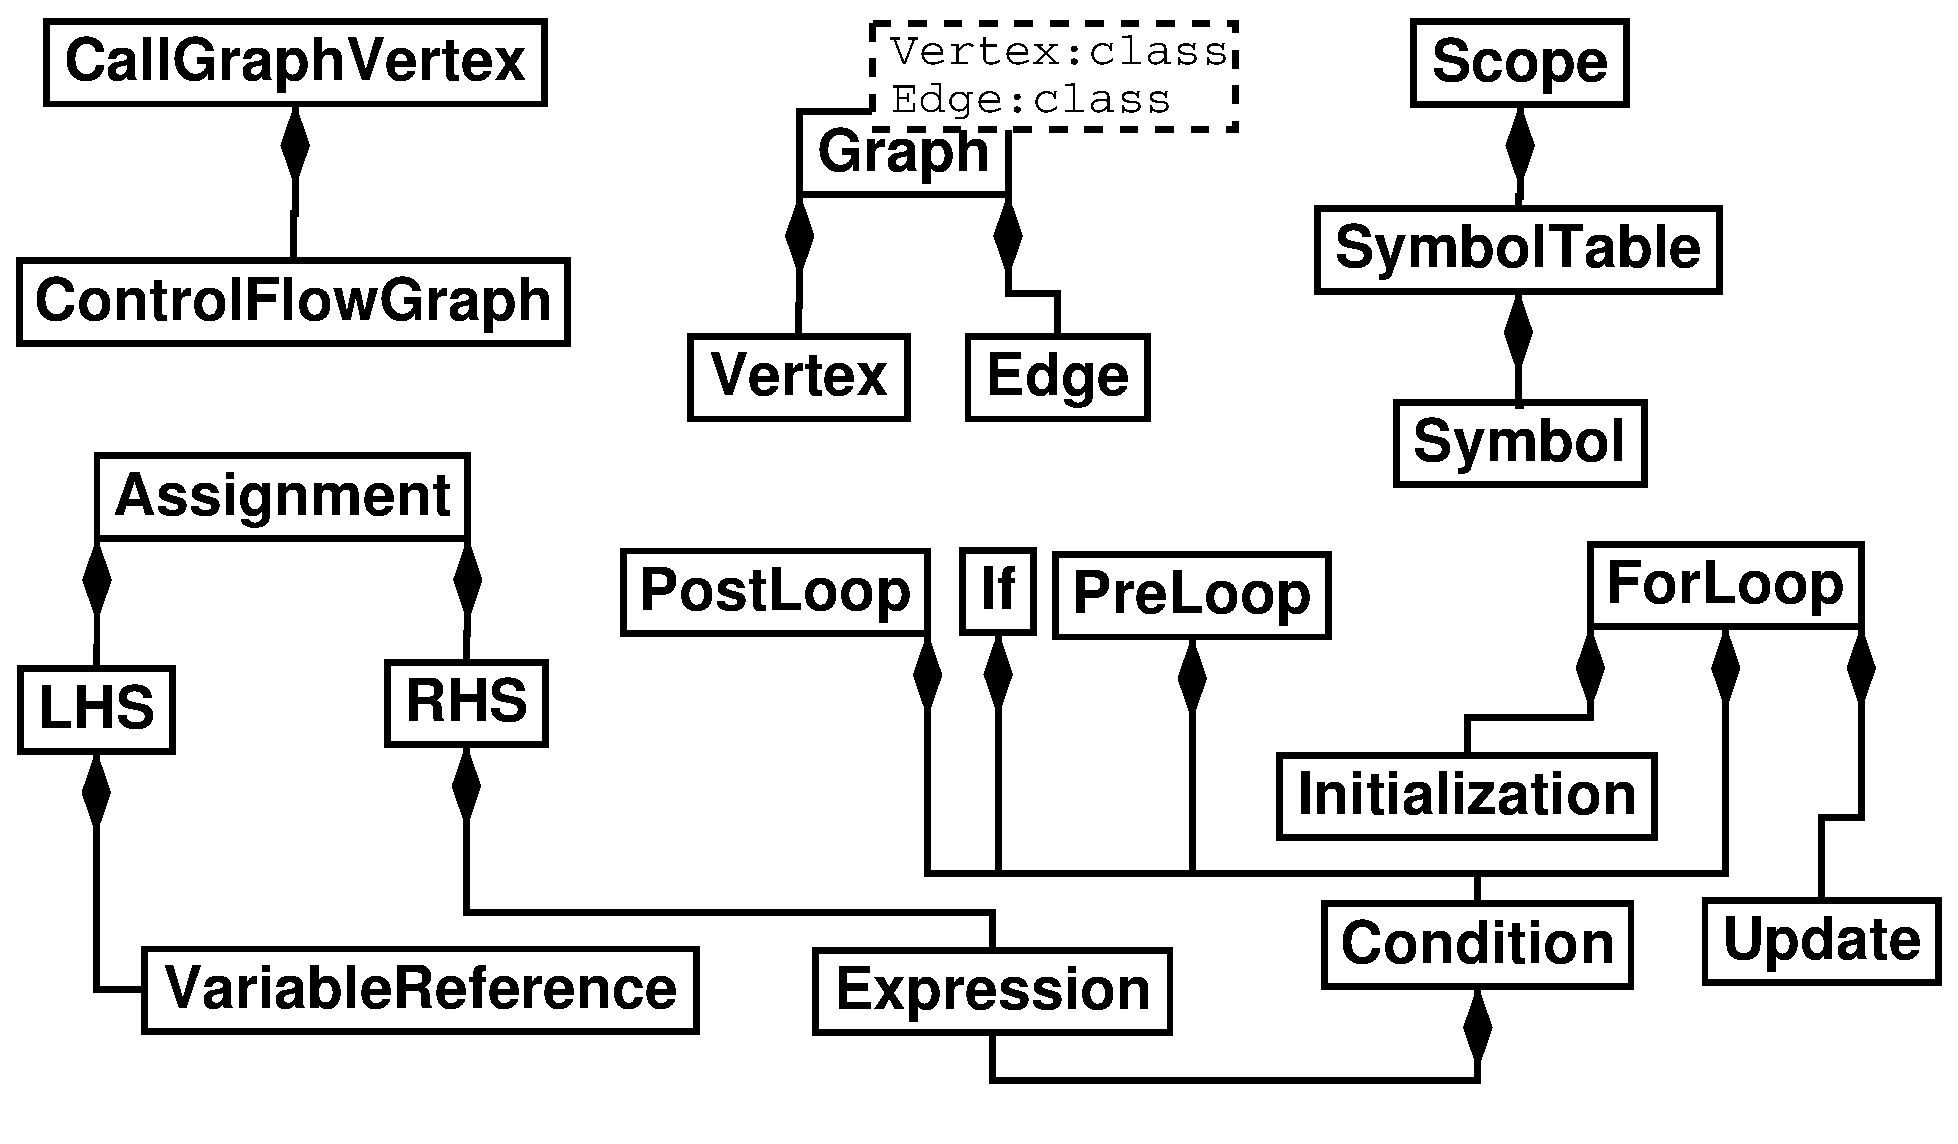
\epsfig{file=irComp.eps,width=.45\textwidth}
\caption{Composition hierarchy} \label{fig:irc}
\end{figure}

A complete documentation of the entire data structure 
can be found on the \OpenAD\ website \cite{openadWeb}.
The class hierarchy is organized top down with 
a single \code{CallGraph} instance as the top element. 
\reffig{fig:irc} shows  a simplified composition hierarchy.
This defines ownership of any dynamically allocated elements as well. Where possible,
the interfaces avoid the need for explicit dynamic allocation of members outside the methods of the 
containing class. Only in cases of containment of polymorphic elements is explicit dynamic allocation 
necessary. In such cases the container class interface indicates the assumption of ownership of 
the dynamically allocated elements being supplied to the container class. An example is the 
graph class \code{Expression} accepting vertex instances that can be \code{Constant}, \code{Intrinsic} , and so forth; 
see also \refsec{ssec:AlgorithmsAndInheritance}.

These transformation algorithms are modularized to enable reuse in different 
contexts. 
\begin{wrapfigure}{r}{.55\textwidth}
\centering 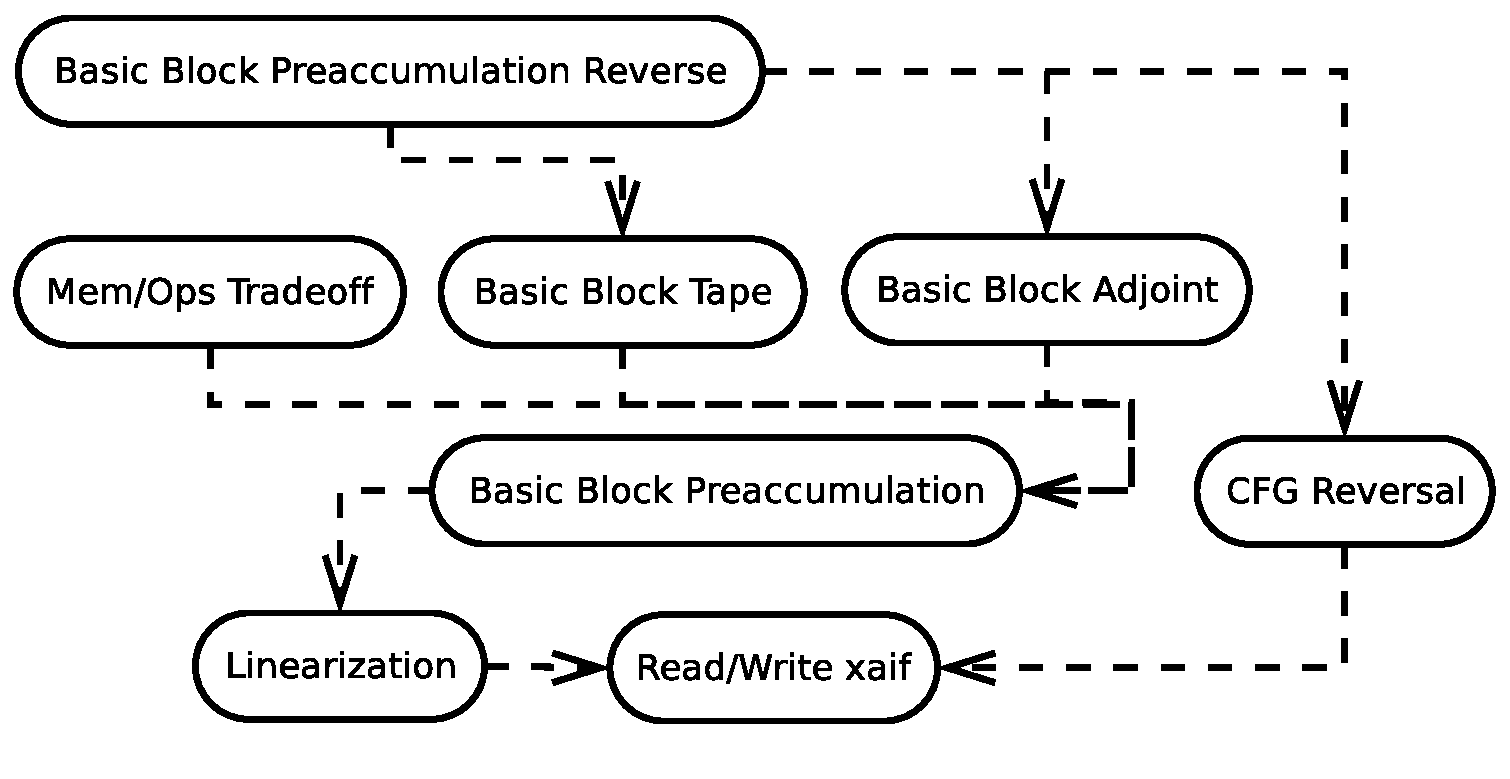
\epsfig{file=allAlgs.eps,width=.45\textwidth}
\caption{\xaifBooster algorithms} \label{fig:allAlgs}
\end{wrapfigure}
\reffig{fig:allAlgs} shows the implemented algorithms with dependencies.
To promote reuse of the transformation algorithms the original data structure 
is never modified. Instead, the data representing modifications or augmentations
are kept in algorithm specific instances that are associated with the 
data structure element that is being modified. 
In the following sections we want to concentrate on the transformation 
the algorithm executes while keeping the technical detail at a minimum. 
 
%-----------------------------------------------------------------------------------------
\subsubsection{Reading and Writing \xaif}
Parsing is done through the Xerces C++ XML parser \cite{xercesWeb}
such that the XML element handler implementations build the \xaifBooster\ data 
structure 
from the top down. 
Aside from the parsing of the actual input \xaif\ there is also the so called 
{\em 
catalogue of inlinable intrinsics
} 
supplied as an XML following a specialed schema in \xaif, see also 
\refsec{sssec:linearization} and \refsec{sssec:wtxxtw}.
As an additional consisency check all components that read \xaif\ data 
have the validation according to the schema enabled. Beyond the schema 
validation these components perform valdity checks. Therefore, 
manual modifications of \xaif\ data , while possible, should 
be done judiciously. 

The unparsing of the transformed data structure into \xaif\ is performed 
through a series of that traverses the data structure and the 
respective algorithm specific data. 
For information of the files containg the \xaif\ representation refer to 
\refsec{ssec:manualPipeline}.

%-----------------------------------------------------------------------------------------
\subsubsection{Linearization}\label{sssec:linearization}

As explained in \refsec{sec:ADIntro} a necessary step is the computation of 
the local partial derivatives $c_ji$ that can be thought of as edge labels 
in the computational graph $G$. Per canonicalization all elemental $\phi$ 
occur in the right-hand side of an assignment. 
For each $\phi$ we look up the definition of the respective partials in 
the intrinsics catalogue. 
{\color{Red} [ not sure  how much detail is necessary ] } 
They are defined in terms of positional arguments. Because of this, 
the right-hand-side expression may have to be split up into 
subexpressions to assign intermediate values to ancillary variables 
that can be referenced in the partial computation.  
{\color{Red} [ a figure here? ] }
In cases of the left-hand-side variable occuring on the right-hand-side (or being 
may-aliased to a right-hand-side variable, see )
The result of the Linearization. 
 


{\color{Blue} [ this is old stuff from the abstract]  
\begin{figure}[htb]
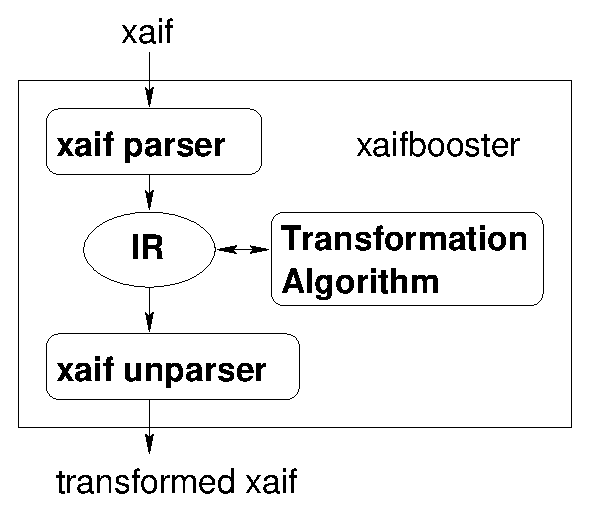
\epsfig{file=principle.eps,width=4cm}
\caption{\xaifBooster\ parses xaif code into an internal representation (IR).
It provides an API for transformation algorithms to modify the IR. An unparser
returns the transformed xaif code.} \label{fig:xaifBooster}
\end{figure}
The C++ code \xaifBooster\ is a collection of utilities and routines for the
(semantic) transformation of programs given in xaif. Its principal architecture 
is illustrated in \reffig{fig:xaifBooster}. One of the major concerns during
the development of \xaifBooster\ has been the clean separation of the internal
representation (an enhanced object image of xaif) from algorithms that operate 
on this data structure. This goal has been achieved by applying the design 
patterns \cite{DesignPatterns} factory, visitor, and decorator as described in \cite{UtNa03}.
The result is an API that gives AD developers the opportunity
to implement new algorithms in a source transformation environment without
having to implement full compiler front- and back-ends. Building on
this API, we have implemented a tangent-linear algorithm that uses statement-
\cite{SEUpreacc} and basic-block-level preaccumulation of local 
gradients/Jacobians. Near-optimal face elimination \cite{ElimTechMP} sequences 
are computed by the software tool 
ANGEL \cite{AGN03,SAGA} ({\tt angellib.sourceforge.net}) and transformed into 
Jacobian code by
an \xaifBooster\ algorithm. A simple adjoint version of the code is obtained
by taping the local Jacobians 
and by computing the corresponding ``transposed Jacobian-vector" products 
during an interpretive reverse sweep through the tape. This approach is
essentially equivalent to split program reversal \cite{Gri00} and allows
for an easy coupling of tangent-linear and adjoint versions of small to 
medium-sized codes as described in \cite{NaHe03}. 

Details of the automatic generation of adjoint code in split mode are presented
in the full version of the paper. Furthermore, additional information is 
provided on \xaifBooster\ as a platform for implementing new AD algorithms with 
the objective to establish an open quasi-standard development infrastructure
within the AD community.
}
%-----------------------------------------------------------------------------------------
\subsection{\OpenAnalysis} \label{ssec:openanalysis}

The \OpenAnalysis\ toolkit, see \cite{oaWeb},  separates program analysis from 
language-specific or front-end specific intermediate representations.
This separation enables a single implementation of domain-specific 
analyses such
as activity analysis, to-be-recorded analysis, and linearity analysis
in  \OpenAD.

{\color{Red} [ what interfaces are there, schema on how it works] } 

{\color{Red} [ It would be nice if this went a little into aliasing ] } 
  

Standard analyses implemented within 
\OpenAnalysis\ such as
CFG construction, call graph construction,
alias analysis, reaching definitions, ud- and
du-chains, and side-effect analysis are available to \OpenAD\ 
via  \OpenADFortTk. 

{\color{Red} [ we can pick an example for an analysis interface 
to show how its done between OA and fortTk and why it makes sense 
that forttk uses OA and not xaifBooster] } 

Activity analysis is performed by \OpenAnalysis based on information
from the Fortran~90 front-end.  The independent and dependent variables of
interest can be communicated to the front-end through the use of pragmas, 
see \refsec{sssec:mfef}.
The results of the analysis are then 
encoded by the Fortram~90 front-end into XAIF.  The analysis indicates
which variables are active at any time, which memory references are active, 
and which statements are active.

The activity analysis itself is based on the formulation in~\cite{UweTBRPaper}.
The main difference is that the data-flow framework in \OpenAnalysis does not
yet take advantage of the structured data-flow equations.  Activity analysis is
implemented in a context-insensitive interprocedural fashion.


%#########################################################################################
\section{Tool Usage}
The following contains brief instructions how to obtain and use \OpenAD. 
While the principal approach will remain the same, future development may 
introduce slight changes. The reader is encouraged to refer to the 
up to date instructions on the \OpenAD\ website \cite{openadWeb}.
\subsection{Download and Build} 
\subsection{Automatic Pipeline}
\subsection{Manual Pipeline}\label{ssec:manualPipeline}


%#########################################################################################
\section{Application}

The reference application for the first prototype of an \OpenAD\ implementation
is a simplified oceanographic box model for investigating
thermohaline circulation. It relates to the
ocean circulation's role in the variability of the climate system,
on time scales of decades to millennia \cite{tzi-ioa:02}.
Previously, the AD tool TAF \cite{GiKa02} 
had been used to generate the derivative
code in both forward and reverse modes.
See \cite{maro-eta:99} for an applications of
TAF's predecessor TAMC to the MITgcm.

\OpenAD\ has been used to generate tangent-linear and 
adjoint versions of the box model. We established numerical identity between
the Jacobians provided by TAF and \OpenAD.
The successful 
application of \OpenAD\ to the box model code is considered as a feasibility 
proof for the overall approach taken by the ACTS project.  
%-----------------------------------------------------------------------------------------
\subsection{Shallow Water Model}
%-----------------------------------------------------------------------------------------
\subsection{Derya's application}
%#########################################################################################
\section*{Conclusion and Future Work}

\OpenAD\ is an AD tool development infrastructure. Its well-separated components
allow developers to focus on various aspects of source-to-source 
transformation AD, including parsing and unparsing of different programming
languages, data and control flow analysis, and (semantic) transformation 
algorithms. The intention of \OpenAD\ is to provide the AD community with 
an open, extensible, and easy-to-use platform for research and development
in the field. Its intention is not to render obsolete existing source transformation
tools such as ADIFOR,\footnote{{\tt http://www.cs.rice.edu/\~\!adifor}} 
the differentiation-enabled NAG Fortran 95 
compiler,\footnote{{\tt http://www.nag.co.uk/nagware/research/ad\_overview.asp}} TAF,\footnote{{\tt http://www.FastOpt.de}} and TAPENADE.\footnote{{\tt http://tapenade.inria.fr:8080/tapenade/index.jsp}} 
Their closer coupling with the language-specific internal representation of 
the program has the potential to make the
exploitation of certain language features easier. \OpenAD\ is supposed to 
complement these tools by providing well-defined APIs to an open internal 
representation that can be used by a large number of AD developers.
Users of AD technology will benefit from the expected wide
variety of combinations of front-ends and algorithms that is made possible
by \OpenAD.

During the remainder of the ACTS project we will focus on the implementation
of robust and efficient data flow algorithms in \OpenAnalysis, including alias, 
define-use and use-define, in-out \cite{Muc97}, 
activity, and to-be-recorded \cite{HNP02} as well as on 
the development of various reverse mode algorithms for parallel MPI codes
combining elements such as preaccumulation and (automatic) checkpointing
\cite{Gri92}. 
A second set of target 
applications in chemical engineering \cite{FTB97} requires combinations of first and 
second derivatives in addition to methods for exploiting structure and sparsity
of the underlying computation. We intend to investigate ways to compute these
combinations efficiently by integrating \OpenAD\ into the relevant 
numerical algorithms.

Ultimately, our aim is to generate correct, efficient, scalable, and easily 
maintainable adjoint code for the MITgcm. The major challenge arises from the
requirement to tackle problems in which derivatives are calculated with respect 
to billions of controls. A combination of the methods outlined above is 
essential to guarantee the successful completion of this highly ambitious
project.

%#########################################################################################
\bibliographystyle{acmtrans}
\bibliography{openad}


\begin{received}
Received May 2005;
\end{received}

\end{document}
